\cleartoverso 
\chaptercontents{Topological Graph Theory}{topgraphchapcover.tikz}{A graph is a set of vertices which are connected by edges. This is a simple example of a topological space. Two topological characteristics of graphs are the number of connected components, and the number of cycles they contain.}

\label{chap:topgraph}
	\begin{elevator}[Basic Definitions]	
A \emph{graph} is a mathematical representation of network. We will explore some basic combinatorial properties of graphs, such as paths and cycles. Here, you can also find the definitions of some commonly used graphs like trees and complete graphs. 
\end{elevator}%
\label{sec:graph:basic}% 
Graph theory is a branch of mathematics that naturally arises when you study a group of objects and a relationship that exists between pairs of objects.
For example, you might be studying a group at a party, and the friendships that exist between pairs of attendees.
Even this simple setting presents itself with some interesting questions, like how tight-knit this group is, or which folks at the party are the least related.
Since this type of structure shows up so frequently in mathematics, we will set up an abstract mathematical object called a graph which contains the mathematical data to describe these types of relationships.
\begin{definition}[Graph]
	A \emph{graph} $G$ is a collection of \emph{vertices} $V(G)$ and a set of \emph{edges} 
	\[E(G)\subset V\times V.\]
	The edge is required to be unordered in the sense that  whenever $(v,  w)\in E(G)$,  the pair  $(w,  v)\not\in E(G)$.
\end{definition}
In the case where the graph $G$ is clear, we will suppress the label and simply denote the vertices  by $V$ and edges by $E$.
\nomenclature{$G$}{A graph}
\nomenclature{$E(G)$}{The edge set of a graph $G$}
\nomenclature{$V(G)$}{The vertex set of a graph $G$}
While this definition gives us the mathematical rigor necessary to begin our explanation of graphs, it is useful to have some good examples in mind to ground our discussion.
%\footnote{I usually have a hard time understanding definitions in mathematics without first drawing a picture. In fact, I suggest that on a first reading of this book to look at the pictures before reading the definitions or proofs.}
\begin{examplefigureenv}[Friends in the Order]{191figures/topgraph_potter.tikz}
Let us look at the motiviating discussion of groups of friends at a party, and see how this fits into the definition of a graph.
Each person in the population would represent a vertex, and the edges between vertices correspond to the pairs of attendees who are friends.
\end{examplefigureenv}
\begin{framedpage}{example}{Some Common Graphs}{It is good to have some examples of graphs in mind before we go around discussing the theory of graphs.}

\begin{smallexamplefigureenv}[Graph:]{191figures/topgraph_graph.tikz}
One way to construct a graph is to build it by hand. 
For example, we can give a graph four vertices and 4 edges by specifying
  \[V=\{1,2,3,4\}\;\;\; E=\{12,23,13,14\}.\]
 While mathematically precise, this presentation is not very intuitive, and so when we want to specify a graph in this text, we will usually just draw a picture of that graph, and assume that it has some explicit (although unwritten) labeling of the vertices and edges.
\end{smallexamplefigureenv}


\begin{smallexamplefigureenv}[Complete Graph:]{191figures/topgraph_completegraph.tikz}
  One especially important family of graphs are the \emph{complete graphs}, which are saturated with edges.
\noindent Let $n\in \N$ be a natural number. The \emph{complete graph on $n$ vertices},  denoted as $K_n$, is the graph with $n$ vertices and an edge between every pair of vertices. 
Since every edge corresponds to a choice of 2 vertices, and in the complete graph we've chosen every pair, it follows that 
\[|E_{K_n}|={n\choose 2}.\]
One reason we call this graph complete is because every graph on fewer than $n$ vertices is a subgraph of $K_n$. 
\end{smallexamplefigureenv}
\nomenclature{$K_n$}{The complete graph with $n$ vertices}


\begin{smallexamplefigureenv}[Octahedron:]{191figures/topgraph_octahedron.tikz}
Graphs naturally arise from other branches of mathematics. 
For example, every polyhedra in $\RR^3$ determines a graph by its edges and vertices. In the diagram on the left, we see the graph corresponding to the octahedron.
Later, we will classify the platonic solids by understanding the combinatorics of their corresponding graphs. 
Notice that a polyhedron has more data than just its underlying graph, as it also knows what combinations of edges and vertices make up faces of the polyhedron. 
\end{smallexamplefigureenv}
\end{framedpage}
A good way to understand a graph is to draw a diagram of it, by placing a  dot for each of the vertices, and drawing a line segment or curve between two vertices if that pair is inside of the edge set $E$. 
The edges of these diagrams are allowed to cross each other, and the edges need not be drawn straight.

Even after introducing a couple of graphs, we can already see some interesting topological properties.
For instance, the complete graph on 5 vertices can only be drawn with edges that cross, whereas every graph that represents a platonic solid can be given by a planar drawing without edges crossing.
Before we get to describing topological properties of graph, let's first describe some of the combinatorial data attached to a graph. 

In this text, the vertices of a graph will be labelled with lowercase letters $u, v, w, x, y.$
For edge, we will either use the letters $e, f$; or we will refer to an edge with endpoints $u$ and $v$ by the pair $uv$. With this notation, we say that $uv$ is an edge if either $(u, v)\in E$ or $(v, u)\in E$. 
\nomenclature{$N(v)$}{The neighborhood of a vertex $v$}
The simplest piece of data that we can ask about a vertex in a graph is the number of neighbors it has.  
\begin{definitionfigureenv}[Neighborhood]{191figures/topgraph_neighborhood.tikz}
	Fix some vertex $v$. Then the subset of vertices which are connected to $v$ by an edge is called the \emph{neighborhood} of $v$, and will be denoted 
	\[N(v):=\{u\in V \;|\; (u,v) \text{ or } (v, u)\in E\}\]
	 The number of edges connected to $v$ is called the \emph{degree} of $v$ and is denoted 
	\[\deg(v):=|\{u \in N(v)\}|.\]
\end{definitionfigureenv}

\nomenclature{$\deg(v)$}{The degree of $v$}
We can already capture a lot of data about a graph simply by knowing the degrees of the vertices in it.
For example, if $|V(G)|=n$, and every vertex has degree $|n-1|$, then it must be the case that $G=K_n$.
If instead every vertex has degree 2, then it must be the case that $G$ is a collection of cycles.
Both of these give us example of  \emph{regular graphs}, which are graphs whose vertices all have the same degree.
A natural family of regular graphs that show up are the Platonic solids.

The degree of a vertex provides \emph{local} information about the graph.
This means that knowing the degree of a particular vertex $v\in G$ doesn't tell us a lot about the graph as a whole --- we only learn about a small portion of the graph around $v$.
This is contrasted with quantities like $|E(G)|$ and $|V(G)|$, which tell us \emph{global} information about our graph. 
In many ways, topology is the study of how local information can be meaningfully assembled into global data. 
\begin{claim}[Average vertex degree]
Let $d(G)$ be the average degree of the vertices of a graph.
The total number of edges in $G$ is:
\[2|E|=d(G)|V|.\]
\label{claim:avgdegree}
\end{claim}
Here, we are using averaging to take local information -- the degree -- and obtaining some information about the entire graph. 
The rough idea of proof is that every edge contributes $+1$ to the degree of each of its ends, so that the sum of all the degrees of the vertices will be twice the number of edges. 
We therefore obtain the equality 
\[2|E|= \sum_{v\in V} \deg(V)= d(G)|V|.\]

But let's try to make this argument a little more mathematically watertight.
%\footnote{As with many mathematical proofs, the outline of the proof is much easier to comprehend than the detailed exposition.
%If you're reading this for the first time, feel free to look at pictures and skip the detailed expositions if you've gotten the gist of the proof.
%Sometimes reading the details just makes the idea of the proof more muddy due to the need to unpack definitions and use notation.}  
\begin{proof}
	From the definition of average degree 
\begin{align*}
d(G)|V|=&\sum_{v\in V}\deg (v)
=\sum_{v\in V} \sum_{u\in V} \delta_E(u,v)+\delta(v, u)
\intertext{where $\delta_E(u,v)=1$ if $(u,v)\in E$, and 0 otherwise. The reason both orders are necessary is because our definition of edge used ordered pairs $(u,v)$.}
=&\sum_{(u,v)\in V\times V} \delta_E(u, v)+\delta_E(v, u)
\intertext{As $\delta(u, v)$ only takes a value of 1 on sets $(u, v)$ that are in $E$, this term counts the number of edges}
=& 2|E|
\end{align*} 
\end{proof}
A good example keep in mind for this lemma are the complete graphs. These $n$-vertices of these graphs each have $(n-1)$ neighbors, so by \sref{claim:avgdegree}  the number of edges in a complete graph is $\frac{n(n-1)}{2}$. 
We also get this strange, but surprisingly useful, corollary. 
\begin{corollary}[An Even number of odd vertices]
	The number of odd degree vertices in any graph is even. 
\end{corollary}
The proof is left to  \sref{exer:evengraph}.
One general mathematical principle is that a large, complicated object (like a graph) can be understood by asking questions about its substructures. 
For instance, by asking how many edges or how many vertices are in a graph, we can begin to get an understanding of its global structure.
In the setting of graphs a particularly useful substructure to study are subsets of the edges and vertices which themselves make \emph{subgraphs} of $G$.
Here are two especially important types of subgraphs which we will look at throughout the course.

\begin{definition}[Paths and Cycles]
	Let $G$ be a graph. A \emph{path} in $G$ is a sequence of distinct vertices $\{v_i\}_{i=0}^n$ such that $v_iv_{i+1}$ is an edge in $G$ for every $i$. The length of the path is the number of edges in it. We say that a path \emph{starts at $v_0$ and ends at $v_k$.} A \emph{cycle} in $G$ is a path $P$ such that the first and last vertex of $P$ share a common edge (which is not already in the path $P$)% \footnote{A word of caution for those who may be using another text; there is some disagreement about whether paths are allowed to repeat vertices or edges. You may see variations of the above definition being called a simple path, or trail, or walk, depending on where you look.}
\end{definition}

Paths and cycles are useful subgraphs to study as they can probe \emph{global} data about the graph.
If you know that a graph has a path between any two points, or that a graph contains no cycles, then you've learned something interesting about the global topological information of that graph.

\begin{examplefigureenv}[Paths and Cycles]{191figures/topgraph_cycle.tikz}
 In the drawn example, we have a path 4 highlighted in red, and a cycle of length 3 highlighted in blue.
The longest path that one can draw would have length 5, and the largest cycle has length 6. 
\end{examplefigureenv}
Since every edge constitutes a very short path, it will necessarily be the case that a non-trivial graph has some paths in it.
However, it need not be the case that a graph have any cycles.
\begin{examplefigureenv}[Trees]{191figures/topgraph_tree.tikz}
	A \emph{tree} is a graph with a unique path between any 2 points. 
	This is a global property of a graph.
	If we fix a vertex $v$ in the tree (called a root), then the set of paths that start at $v$ are in bijection with the vertices in the tree.
	In \sref{exer:tree}, several different interesting properties of a graph are shown to be equivalent to being a tree. 
\end{examplefigureenv}
The length of the longest path in a graph $G$ is telling us something about the global structure of the graph-- you need to look at the entire graph to find the longest path.
As before, we look at how we can assemble local information -- in this case, the degrees of the vertices -- to provide some information on this invariant.
\begin{claim}
	Let $\delta$ be the minimal degree of the vertices in $G$. Then $G$ has a path of length $\delta$. 
\end{claim}	
\begin{proof}
	Start with any path $P$.
	% \smarginnotel{\margingraphics{191figures/topgraph_minpath}} 
	Let $\{v_i\}$ be the vertices of the path.
	Let's look at initial vertex of the path , $v_0$. 
	Suppose that we can find a vertex $w\in N(v)$, which is not already contained within the path $P$. 
	Take this vertex $w$, and append it onto $P$ to build a new path $wP$ which is one vertex longer.

	We can continue this process unless we've grown our initial path to a path  $P'$ which can no longer be extended. This will happen if every point in the neighborhood of the end of the path is contained within the path.  
	For this path $P'$, we have $N(v_0)\subset V(P')$.
	Since $\delta \leq |N(v_0)|<|V(P)|$, we conclude that $\delta \leq |E(P)|$. 
\end{proof}
\begin{elevator}[Connectivity]
	A graph is connected if you can travel between any two vertices along the edges of the graph. We also look at several different quantitative measurements of connectivity.
\end{elevator}
\label{sec:graph:connectivity}
Topology is the study of mathematical structures which have a notion of how their parts are connected to eachother.
A graph is an example of a topological structure, as each vertex ``knows'' which neighbors it is connected to. 
By travelling from vertex to vertex along edges, we can explore questions about the global connectivity of a graph.

\begin{definitionfigureenv}[Vertex Connectedness]{191figures/topgraph_disconnectingset.tikz}
	A graph $G$ is called \emph{connected} if for any two vertices $v$ and $w$,  there exists a path from $v$ to $w$. 
	A disconnecting set $U\subset V$ is a set of vertices with the property that the graph $G\setminus U$ is disconnected.
	The \emph{connectivity of $G$}, denoted $\kappa(G)$, is the size of the smallest disconnecting set of $G$.  
\end{definitionfigureenv}

The connectivity of a graph is an important measurement for applications.
For example, if we are building a power grid for a utility, then whether or not the power can be delivered to the entire network from a single node is determined by the connectedness of the underlying graph. 
The connectivity of the network is a slightly stronger measure, which tells us the maximal number of nodes of the network can fail and still have the network remain connected.
We have a property of a graph which interpolates between the connectivity number and the connected property. We say that a graph is $k$-connected if no vertex set of size $k$ disconnects the graph $G$.
Equivalently, a graph is $k$-connected if its connectivity is at least $k$. 

%\begin{figure}
%	\centering
%	
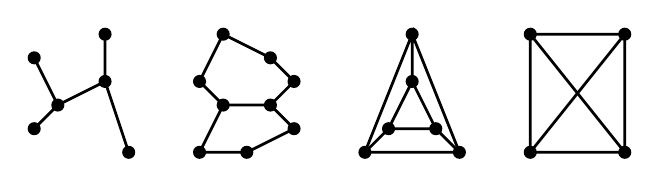
\begin{tikzpicture}[scale=.3]
    \newcommand{\vertexradius}{2.5pt}
\newcommand{\vertexscale}{.5}
\newcommand{\bigvertexscale}{1}
\newcommand{\vertex}{\node[circle, fill=black, scale=\vertexscale] }
\newcommand{\highlighta}{red!20}
\newcommand{\highlightb}{blue!20}
\newcommand{\highlightc}{green!20}
\newcommand{\shadinga}{gray!20}
\newcommand{\smallvertex}{\node[circle, fill=black, scale=.2]}
\newcommand{\highlightlinewidth}{3pt}

\tikzset{every path/.style={line width=1 pt}}
\vertex at  (14,5){};
\vertex at  (9,1) {};
\vertex at  (7,0) {};
\vertex at  (5,0) {};
\vertex at  (9,3) {};
\vertex at  (8,4) {};
\vertex at  (8,2) {};
\vertex at  (6,2) {};
\vertex at  (5,3) {};
\vertex at  (6,5) {};
\vertex at  (2,0) {};
\vertex at  (-2,1){};
\vertex at  (1,3) {};
\vertex at  (-1,2){};
\vertex at  (1,5) {};
\vertex at  (-2,4){};
\vertex at  (23,5){};
\vertex at  (23,0){};
\vertex at  (19,5){};
\vertex at  (19,0){};
\vertex at  (16,0){};
\vertex at  (15,1){};
\vertex at  (14,3){};
\vertex at  (13,1){};
\vertex at  (12,0){};
\draw (1,5) -- (1,3)  -- (2,0);
\draw (-2,1) -- (-1,2) -- (-2,4);
\draw (-1,2) -- (1,3);
\draw (6,5) -- (5,3) -- (6,2) -- (8,2) -- (9,3) -- (8,4) -- (6,5);
\draw (6,2) -- (5,0) -- (7,0) -- (9,1) -- (8,2);
\draw (14,3) -- (13,1) -- (15,1) -- (14,3);
\draw (14,3) -- (14,5) -- (12,0) -- (16,0) -- (14,5);
\draw (12,0) -- (13,1);
\draw (15,1) -- (16,0);
\draw (19,5)  -- (19,0) -- (23,0) -- (23,5) -- (19,5) -- (23,0);
\draw (19,0) -- (23,5);
\pgfsize \end{tikzpicture}


%	\caption{Graphs with connectivity 1, 2, 3, and 4. }
%\end{figure} 


\begin{examplefigureenv}[Bottlenecks and Connectivity]{191figures/topgraph_risk.tikz}
	If $H\subset G$ is a subgraph, one can measure the size of the smallest set it takes to disconnect $H$ from the remainder of $G$.
	This will always be at least the connectivity of the entire graph.
	In the game of \emph{Risk}, the continent of Australia is especially prized because of it's low vertex connectivity to the remainder of the graph. 
\end{examplefigureenv}

\nomenclature{$\kappa(G)$}{The vertex connectivity of $G$}
Connectivity has a strange relationship with topology.
Whether or not a graph is connected is a \emph{topological} property of the graph. However, the connectivity of a graph is \emph{not} a topological property.
An example that demostrates that connectivity is not a topological property are the graphs of the triangle and the square, which are topologically indistinguishable.
However, the triangle is three connected, and the square is only 2 connected! We will later see in \sref{sec:graph:Minors} exactly why connectivity is not a topological property. 
You can observe that even making small modifications to the graph (like making the edge of a graph into a path,) can greatly change to the connectivity of a graph. 

It is possible to get an estimate on the connectedness of an average component of the graph by knowing the average degree of the vertices of a graph.
In short, if you have a lot of edges, then we expect the graph have a connected component with high connectivity (see \sref{graph:thm:mader}.)


\begin{framedpage}{theorem}{Mader's Theorem}{Every graph with average vertex degree $d(g)$ greater than $4k$ contains a $k$-connected subgraph. \label{graph:thm:mader}}
	The idea of this proof is to induct on the number of vertices, where the vertex we remove during the inductive step is one of low degree. We start by massaging $d(G)\geq 4k$ to obtain the inequalities
	\begin{align*}|V|\geq 2k-1 && |E|\geq (2k-3)(|V|-k+1)+1\end{align*}
	For the first inequality, notice that if the average degree is $4k$, there must be a vertex with degree at least $4k$; therefore it has $4k$ neighbors. Therefore the number of vertices is at least $4k$. 
	For the second inequality, we apply \sref{claim:avgdegree},
	\[|E|= d(G)|V| \geq  4k  |V| 
	\geq(2k-3)(|V|-k+1)+1\]
	With these two new inequalities, we run an inductive argument on the number of vertices in the graph. In the base case, $G$ is a graph on $2k-1$ vertices and therefore is complete, for which the claim follows trivially.

    For the inductive step, we split into two cases based on whether there exists a vertex of low-degree. If $v$ has low degree, then $G\setminus v$ will have \emph{larger}  average degree, and by induction we can still run our argument. 
    
	\textbf{Case 1:} Suppose that there exists a vertex of degree less than $2k-3$. Then even after removing this vertex, our inductive hypothesis holds as we've decreased the number of vertices by 1 but only removed at most $(2k-3)$ edges.
\begin{paragraphfigureenv}[]{191figures/topgraph_disconnect.tikz} 
	\textbf{Case 2:} Suppose that the inequality is not sharp,  and we cannot find a vertex of degree $2k-3$ or less. Let's assume for contradiction that $G$ is not $k$-connected. Then there are two subgraphs $G_1,  G_2\subset G$ such that $G_1\cap G_2$ has fewer than $k$ vertices. 
	Every vertex in $G_1\setminus G_2$ has neighbors only in $G_1$. Since the minimal degree of each vertex is $2k-2$,  we have that $G_1$ has at least $2k-1$ vertices. Similarly,  $G_2$ has $2k-1$ vertices. So, both the graphs $G_i$ satisfy the first inequality for our induction hypothesis.
	\end{paragraphfigureenv} As $E=E_1\cup E_2$, we get $|E|\leq |E_1|+|E_2|$. We additionally know that $|V_1|+|V_2|\leq |V|+k$. Combining these inequalities gives
	\[(2k-3)(|V_1|-k+1)+1)+(2k-3)(|V_2|)-k+1)\leq (2k-3)(|V|-k+1)+1\leq |E|\leq |E_1|+|E_2|\]
	from which we conclude that one of the $G_i$ satisfy the induction hypothesis, and therefore contains a $k$-connected subgraph. 
\end{framedpage}

There is no particular reason why we choose to use deletion of vertices to define the connectivity of a graph. 
We could have instead used edges to get a measure of connectivity, and define the \emph{edge connectivity} as the minimal number of edges that you must remove to disconnect the graph.
Somewhat surprisingly, the vertex connectivity and the edge connectivity are usually not related to each other.
\begin{examplefigureenv}[Dumbbell Graph]{191figures/topgraph_dumbbell.tikz}
Consider the dumbbell graph which is created by taking two $K_n$ and mutually connecting them to a new vertex $v$. 
In order to disconnect this graph by removing edges, you need to remove at least $n$ edges.
However, to vertex disconnect the graph, it suffices to take out the middle vertex $v$.
\label{fig:graph:dumbell}
%See Exercise \sref{exer:edgeconnectivity} for a basic bound. 
\end{examplefigureenv}
The discrepancy between the edge and vertex connectivity is due to the fact that a concentrating edges onto a single vertex gives it low vertex connectivity, but has little impact on edge connectivity.


\begin{projectdescription}{Spectral Graph Theory}
A more quantitative measure of connectivity examines the average distance squared between two vertices in the graph.\label{proj:spectral}
We now give a nice algebraic characterization of this metric. 
Let  $V=\{v_1, \ldots, v_n\}$ be the vertices of a graph $G$. 
The \emph{adjacency matrix of $G$}  is the $n\times n$ matrix $A$ whose $ij$ entry is $1$ if $v_iv_j$ is an edge, and $0$ otherwise.
Define the \emph{degree matrix} $D$ to be the diagonal matrix whose $i$th diagonal entry  is $\deg(v_i)$.
Finally, we define the \emph{Laplacian} of the graph $G$ to be the matrix 
\[
	L=D-A.
\]
The eigenvalues of $L$ bound the connectivity of $G$, and in applications gives a more nuanced definition for connectivity.
\end{projectdescription}

As demonstrated by the dumbell graph (\sref{fig:graph:dumbell}), the vertex connectivity tells us where the bottlenecks are in our graph. 
Another way of counting the bottlenecks in a graph would be to ask how many independent paths there are betweeen two vertices, as the presence of a bottleneck in the graph will force this number to be small.
\begin{definition} [$k$-path connected]
	A graph is \emph{$k$-path connected} if any two vertices $v$ and $w$ can be joined by at least $k$ disjoint paths. 
\end{definition}
You can check that  the dumbell graph (\sref{fig:graph:dumbell}) is only 1-path connected, as there is only one way to get from the left portion of the graph to the right portion. Menger's theorem (\sref{graph:thm:mengers}) tells us that this is generally the case: the path connectivity of a graph is equal to its vertex connectivity.

Menger's theorem seems a bit strange on first reading because of a contrast in the definition of path connectedness and vertex connectedness. 
The path connectivity looks to  \emph{maximize} a set of independent paths, while the vertex connectivity is tries to  \emph{minimize} the size of a disconnecting set.

\begin{projectdescription}{Max-Min}
These types of statements are common in combinatorics related to optimization.
Max-Min properties extend to many combinatorial  \label{proj:maxmin}  objects beyond graphs,  and the Max-Min principle has several statements which are all relevant to optimization of networks.  Some equivalent theorems to Menger's theorem include the Max-flow Min-cut theorem, K\"onig's theorem, Dilworth's theorem, and Hall's theorem.
\end{projectdescription}


One application of Menger's theorem is to classify the structure of graphs with connectivity $2$.
\begin{lemma}[Adding paths preserves $\kappa(G)\geq 2$]
	Suppose that $\kappa(G)\geq 2$.
	 Let $v,w$ be two vertices in $G$. 
	Create a new graph, $G\cup_{v,w} P$ by attaching a path of length at to $G$, whose endpoints are $v$ and $w$. 
	Then $\kappa(G\cup_{v, w}P)\geq 2$.\\
	If additionally we require that the path have at least 3 vertices, then $\kappa(G\cup_{v, w}P)=2$. 
\end{lemma}
\begin{proof}
	Suppose for contradiction that $\kappa(G\cup_{v, w}P)=1$. Then there is a disconnecting vertex $u$ so that $G\cup_{v, w}P\setminus \{u\}$ is disconnected.
	It must be the case that $u\in P$, as otherwise $G\setminus \{u\}$ would be disconnected, contradicting that the 2-connectivity of $G$. 
	If $P$ has only two vertices, $\{v, w\}$ we are done (as every candidate vertex for $u$ needs to lie outside of $G$, but $V(G\cup_{w,v}P)=G(P)$. Therefore the length of $P$ must be at least 2. The removal of $u$ from  $P$ separates the path into two 2 components. 
	Each of those components is connected to $G$ by their ends, and therefore $G\cup_{w,v}P\setminus\{u\}$ is still connected.
	$u$ fails to be a disconnecting vertex for $G\cup_{w,v}P$, contradicting our assumption. 

	It remains to show that if the length of $P$ is at least 2, that there exists a disconnecting set for $G\cup_{w,v}P$ of size 2. Observe that $G\cup_{w,v}P\setminus\{w, v\}$ is disconnected if there are any vertices in $P$ besides $w$ or $v$. 
\end{proof}

\begin{doubledpage}{theorem}{Menger's Theorem}{
	The path connectivity of a graph is equal to the vertex connectivity of the graph.  }
\label{graph:thm:mengers}
We first show that the path connectedness is at most the vertex connectedness. 
Suppose that  $v_1, \ldots, v_k$ form a disconnecting set which separates $G$ into two components $G_1$ and $G_2$.
Pick a vertex $u_1\in G_1$, and $u_2\in G_2$.
There can be at most $k$ disjoint paths between $u_1$ and $u_2$, as each path must use one of the $k$ points in the intersection.
This shows that the path connectivity is less than the vertex connectivity.
\begin{paragraphfigureenv}[Setup:]{191figures/topgraph_mengersetup.tikz} To show that the path connectedness is at least the vertex-connectedness, we will prove a stronger statement.  Suppose that $G$ is $k$-connected,  and let $A$ and $B$ be disjoint subgraphs of $G$.
We will show that whenever we have a collection of fewer than $k$ disjoint paths from $A$ to $B$, we can find a larger connection of disjoint paths from $A$ to $B$. Let's set up some notation for this. 
\end{paragraphfigureenv}
\begin{claimfigureenv}[Inductive statement for Menger's Thm.]{191figures/topgraph_mengersetup2.tikz}
Suppose that $A$ and $B$ are subgraphs of $G$ each containing at least $k$ vertices.
Let $b_1, \ldots, b_n$ be vertices of $B$, with $n<k$. 
Let $\mathcal P_n=\{P_1, \ldots , P_n\}$ be a collection of disjoint paths $G$, which 
\begin{itemize}
    \item only intersect $A$ at their left endpoints,
    \item only intersect $B$ at their right endpoints, which are the specified vertices $b_i$. 
\end{itemize}
Then there exists a point $y\in B$ and  collection $\mathcal P_{n+1}$ of $n+1$ disjoint paths in  $G\setminus (A\cup B))$ which satisfy the above conditions, with right endpoints $b_1, \ldots, b_n, y$. 
\end{claimfigureenv}

We will prove this by inducting  on the size of $G\setminus B$. When $B$ is all of $G\setminus A$, then each path $P_i$ consists of a single edge, and $k$-connectedness gaurentees that $A$ cannot be separated from $B$ by fewer than the removal of $k$-vertices.
For our inductive step, let us assume that the claim holds for every subgraph $B'$ containing $B$.  Let's look at our current graph and subgraph $B$. 
Now, we will randomly construct a new path $Q$ from $A$ with a  random endpoint in $B$.
If this path is disjoint from the $\mathcal P_n$, then we are done.
Now, we use the inductive hypothesis by expanding the subgraph $B$ to include a point from the path $Q$. Let $x$ be the final point where the path $Q$ intersects the collection $\mathcal P_n$, and without loss of generality we will assume that $x$ lies on the path $P_n$.
\begin{paragraphfigureenv}{191figures/topgraph_mengersetup3.tikz}
     Denote by $Q_y$ the segment of $Q$ going from $x$ to $y$, and $Q_b$ the segment of $Q$ going from $x$ to $b_n$.  Now  enlarge $B$ by including the path $Q_b$ and $Q_y$, 
\[B':= B\cup Q_b\cup Q_y.\]
The end points $b_1, \ldots, b_{n-1}, x$ satisfy the conditions of the claim.  By our inductive hypothesis, there exist disjoint paths $\mathcal P_{n+1}'$ going from $A$ to end points $b_1, \ldots, b_{n-1}, x, z$ in $B'$. 
\end{paragraphfigureenv}

At this point we've found a subgraph $B'$ containing $B$, and we would like to reduce down to $B$.
We break into different cases based on the location of the point $z$. 

\begin{paragraphfigureenv}{191figures/topgraph_mengercase1.tikz}
    \textbf{Case 1:} In the easy case, $z$ belongs to our original set $B$. In this case, replace $y$ by $z$ in the original step. The paths $P_1', \ldots P_{n-1}'$ and $P_{n+1}'$ with endpoints $b_1, \ldots, b_{n-1}, z$ are disjoint. To create a final path with endpoint on $b_n$, we take the concatenation of the path $P_{n}'$ with endpoint $x$, and the path $Q_b$. Since $Q_b\subset B'$, it is disjoint from all of the $P'_i$ we've constructed so far. This gives us the collection $\mathcal P_{n+1}$ 
\end{paragraphfigureenv}
The more difficult case is when  $z$ only belongs to the enlargement  $B'$. Then $z\in B'\setminus B = Q_b\sqcup Q_y$. By construction, the paths $Q_b$ and $Q_y$ are disjoint, so either $z\in Q_b$ or $z\in Q_y$. 
\begin{paragraphfigureenv}{191figures/topgraph_mengercase2.tikz} \textbf{Case 2a}
    Suppose that $z\in Q_y$. Then consider the paths 
    \begin{itemize}
        \item $P''_n$, which is $P'_n$ concatenated with $Q_b$, and 
        \item $P''_{n+1}$, which is $P'_{n+1}$ concatenated with the portion of $Q_y$ lying after $z$. 
    \end{itemize} 
    These two paths are disjoint from the $P'_1, \ldots, P'_{n-1}$, and are additionally disjoint for eachother. These paths are seen to have interior vertices which are disjoint from $B$, and by construction have left endpoints in $A$. The $\{P_1', \ldots, P'_{n-1}, P''_n, P''_{n+1}\}$ satisfy the conditions of the claim. 
\end{paragraphfigureenv}

\begin{paragraphfigureenv}{191figures/topgraph_mengercase3.tikz}
    \textbf{Case 2b}
     Alternatively, it may be the case that $z$ lies on the path $Q_b$. T
     \begin{itemize}
         \item $P''_n$, which is $P'_{n+1}$ concatenated with $Q_b$, and 
         \item $P''_{n+1}$, which is $P'_{n}$ concatenated with the portion of $Q_y$ lying after $z$. 
     \end{itemize}  
     As in the previous case, the paths $\{P_1', \ldots, P'_{n-1}, P''_n, P''_{n+1}\}$ satisfy the conditions of the claim.
\end{paragraphfigureenv} 
\end{doubledpage}
This gives us a method to build larger 2-connected graphs from smaller 2-connected graphs.
This can be strenghthend to a characterization of $2$-connected graphs. 
\begin{theorem}[Characterization of 2-connected graphs]
	Let $G$ be a 2-connected graph. Then either 
		\begin{itemize}
			\item 
			There is a 2-connected graph $H$ so that $G$ may be obtained by attaching a path of $H$ and
			\[G=H\cup_{v,w} P.\]
			\item 
			$G$ is a cycle.
		\end{itemize} 
\end{theorem}
\begin{proof}
	Suppose that $G$ is not a cycle.
	Since $G$ is 2-connected, $G$ contains at least a cycle.
	This means that $G$ contains a 2-connected subgraph, and so we can find a maximal 2-connected proper subgraph $H$. 
	Here, maximal means that there does not exist another proper 2-connected subgraph $H'$ containing $H$. 
	We would like to show that $G$ is obtained by attaching a path onto the graph $H$. 


	Look at a vertex $v\in G\setminus H$, and a vertex $w\in H$.
	As $G$ is 2-connected,  Menger's theorem ensures that there exists disjoint paths $P_1, P_2$ from $v$ to $w$.
	This gives two paths from $w$ to that are contained in $H$.
	$H\cup P$ is a 2-connected subgraph of $G$.
	It cannot be the case that $H\cup P$ is a proper subgraph, because $H$ was assumed to be the maximal proper 2-connected subgraph of $G$.
	It must then be the case that $G=H\cup P$, concluding the proof. 
\end{proof}
This gives us way to build up all 2-connected graphs. 
\begin{corollary}
	Every 2-connected graph is generated from a cycle with the subsequent addition of paths.
\end{corollary}
We will have to develop a few more tools before we're able to get  a classification result for 3 connected graphs, and will return to this in \sref{sec:graph:3connected}.

 
	\begin{elevator}[Minors and Topological Minors]
Subdivision and contraction are two dual operations which  modify a graph at an edge.
We'll look at how these operations preserve and modify the topological and combinatorial properties of a graph.
\end{elevator}
\label{sec:graph:Minors}
The main goal of topology is to understand what kinds of topological spaces are out there, and classify them.
This means not only understanding how to construct topological spaces, but also when two different spaces are equivalent.
So far, we've been using graphs as the building blocks for topological spaces.
\begin{examplefigureenv}{191figures/topgraph_differentpresentation.tikz}
	When we draw a graph,  we do not care how we draw the edges of the graph --  the edges are allowed to be bent, or straight or cross. Only the adjacency relations between those edges and vertices matter to us.
	For example, both the pentagon and the star drawn represent the same graph, just drawn differently in the plane.
	They also represent the same topological space: both are a combinatorial representation of the circle, $S^1$.
	\end{examplefigureenv}
Before we understand when two graphs represent the same topological space, we should understand when two different graphs are equivalent.
\nomenclature{$S^n$}{The $n$-dimensional sphere}
\begin{definition}[Graph Isomorphism]
	We say that two graphs $G$ and $H$ are \emph{graph isomorphic} if there exists a bijection $\phi: V(G)\to V(H)$ so that whenever $vw$ is an edge of $E(G)$, then $\phi(v)\phi(w)$ is an edge of $E(H)$. 
	\label{def:graphiso}
\end{definition}

Isomorphism is an equivalence relation on graphs. 
Figuring out if two graphs are graph isomorphic isn't an easy task -- proving that there does not exist a map between two graphs can be very tricky. 
Usually, we prove the non-existence of an isomorphism between two graphs by assigning \emph{invariants or properties} to our graphs which only depend on the isomorphism class of a graph. 
This allows us to distinguish non-isomorphic graphs. 

A simple invariant would be to count the number of edges in a graph.  clearly two graphs cannot be graph isomorphic if they have a different number of edges or vertices.
However, there are plenty of graphs which have the same number of edges and vertices and are not isomorphic. 
For example, all trees on $n$-vertices  have $n-1$ edges, and all appear the same when only looking at the number of edges and number of vertices. 

The properties of the graph that we have studied so far (connectivity of a graph, maximal vertex degree) all can be used to distinguish graphs, and when we develop new properties and invariants throughout this course, I encourage you to construct pairs graphs which can be distinguished by the invariant, and pairs of graph which are non-isomorphic but are not distinguished by the property being discussed. 
\begin{projectdescription}{Graph Homomorphisms}
One could weaken the notion of isomorphism to homomorphism, which drops the \label{proj:graphhomo} requirement of \sref{def:graphiso} that the map of vertices be in bijection.
A typical example of a graph homomorphism comes from subgraphs, where one can express the subgraph inclusion  $H\subset G$ via an injective graph homomorphism from $H$ to $G$. 
Asking whether or not there exists a graph homomorphism between two graphs is not only interesting as a relation between graphs, but can be used to construct invariants between graphs.
For example, the graph homomorphisms from $G\to K_n$ can be used to understand the vertex colorings of the graph $G$. 
\end{projectdescription}

\subsection{Subdivision and Topological Minors}

Graph isomorphism does not describe the whole entire story of topological equivalence. 
To a topologist, there is no difference between a path and an edge-- they both describe ``things that look like lines.'' 
In the same light, all cycles, no matter their size, topologically describe the circle. 
While all graph equivalences give us topological equivalences, the notion of topological equivalence is weaker and a bit more nuanced. 
One approach to understanding topological equivalence of graphs is to develop some operations which modify a graph, but keep the topology the same.
\begin{definitionfigureenv}[Subdivision]{191figures/topgraph_subdivision.tikz}
	Let $G$ be a graph,  and let $e$ be an edge in $G$, with endpoints $w_-$ and $w_+$. 
	The \emph{subdivision} of $G$ at $e$ is the graph $G\div e$,  whose vertex set has an additional vertex
	\[
		V(G\div e)=V(G)\cup\{v_e\}
	\]
	and whose edge set connects this new vertex connecting to the ends of $e$:
	\[
		E(G\div e )=V(G)\setminus \{e\}\cup\{v_ew_-, v_ew_+\}.
	\] 
\end{definitionfigureenv}
If $H$ is obtained from $G$ by a sequence of subdivisions,  we say that $H$ is a subdivision of $G$. If a subdivision of $G$ is contained in $H$,  we say that $G$ is a \emph{topological minor} of $H$. The set of all graphs that contain $G$ as a topological minor is denoted $TG$.

	\nomenclature{$G\div e$}{The subdivision of $G$ at $e$} 
While the definition of subdivision may look intimidating, it is a visually intuitive process.
One starts with a graph, selects an edge, and then adds a new vertex into the middle of that edge. 

Every cycle is a subdivision of the basic cycle on 3 vertices. Subdividing any edge of a cycle produces the next larger cycle, so one may say that whenever $m<n$, $C_m$ is a topological minor of $C_n$. The set of graphs whose topology matches that of the circle can be described using subdivisions as $TC_3$. 

\begin{examplefigureenv}[$K_5$ Subdivision]{191figures/topgraph_k5subdivision.tikz}
Graphs contain many more graphs as topological minors than subgraphs.
Notice that every subgraph is a topological minor, but it is usually not the case that a topological minor is a subgraph.
The graph drawn on the right is a subdivision of $K_5$, obtained by taking every edge and subdividing it.
Since this graph is a subdivision of $K_5$, it contains every graph on five vertices as a topological minor.
However, it does not even contain a triangle as a subgraph. 
In fact, every cycle in this graph has even length, which is a pretty uncommon property for a graph to have. 
\end{examplefigureenv}

From a combinatorial perspective, subdivision is a bit confusing.
It doesn't preserve many graph invariants: for example, whenever one subdivides a graph, the vertex connectivity of the graph is reduced down to at most two. 
While things like the maximal degree of a vertex are preserved, almost every other combinatorial properties (like edge or vertex connectivity, coloring) is thrown out of the window. Furthermore, subdivision only serves to make a graph more complicated by adding in additional vertices and edge. 

However, subdivision satisfies all the condition that we value as topologists: when you subdivide an edge, you are allowed to stretch paths out, but  not allowed to break them or create new ones. We will therefore say that the \emph{topological} properties of a graph are those which are preserved under subdivision.
If $H$ is a subdivision of $G$, we will write $G\Rightarrow H$. 

This doesn't form an equivalence relation on graphs, as the relation is rarely reflexive: if $G\Rightarrow H$ then $H\Rightarrow G$, it must be the case that $G=H$. 
However, there is a general trick for constructing equivalence relations out of operations which do not satisfy the reflexive axiom. 

\begin{claimfigureenv}[Homeomorphic]{191figures/topgraph_commonsubdivision.tikz}
Graphs $G_1$ and $G_2$ are \emph{homeomorphic} or \emph{topologically equivalent} if there exists a \emph{common subdivision} $H$ so that 
\[G_1\Rightarrow H \text{  and  } G_2\Rightarrow H.\]
We then write $G_1\simeq G_2$. 
Homeomorphism is an equivalence relation. 
\end{claimfigureenv}
\begin{comment}
Not all kinds of topological deformations are captured by the subdivision relation. Perhaps the most important of these relations is the homotopy equivalence, which is not characterized by subdivision. If we allow for homotopy-like deformations, then a graph is completely characterized by the number of independent loops it has, and so every graph can be homotoped to a graph with one vertex of high degree, and many other vertices of degree 2. However, subdivision preserves more properties than this:
\begin{claim}
Let $H$ be a subdivision of $G$. Then for every $k$, the number of vertices of $G$ of degree $k$ is equal to the number of vertices of $H$ of degree $k$. 
\end{claim}
\end{comment}
As a general rule, subdivision preserves the topological properties of a graph, but loses a lot of the combinatorial data. 
In particular, the operation of subdivision takes a graph $G$, and produces a slightly sparser, more complicated graph $G\div e$.
This means that the operation of subdivision is not particularly useful for proof techniques. 
In short: subdivision is good for topologists, but bad for graph theory.

\subsection{Contraction and Minors}
A slightly more aggressive type of graph deformation is contraction along and edge, which one can use to invert the operation of subdivision. 
\begin{definitionfigureenv}[Contraction]{191figures/topgraph_contraction.tikz}
  Let $G$ be a graph, and let $e$ an edge in $G$ with ends $w_+$ and $w_-$. Then define the \emph{contraction} $G/e$  to be the graph with a new vertex $v_e$ 
  \[
	  V(G/e)=V(G)\setminus \{v_-, v_+\}\cup\{v_e\}
\]
  whose edges are given by neighbors of $e$,
  \[
	  E(G/e)=E(G)\cup\{v_ev \;|\; e\in N(w_-)\cup N(w_+)\}.
	\]
   A graph $G$ is a  \emph{minor} of $H$ is $G$ is a subgraph of a contraction of $H$.
   When $G$ is a minor of $H$, we write $G\preceq H$. 
\end{definitionfigureenv}
\nomenclature{$G/e$}{$G$ contracted along an edge $e$}

The graph $G/e$ is in some sense ``simpler'' than the graph $G$ in that $G/e$ has fewer edges and vertices than $G$. 
Contraction is an opposite operation to subdivision, in that every subdivision can be undone by a contraction. 
However it is not the case that every contraction can be undone by a subdivision. 
For instance, the contraction given in the above example is not a contraction which can be undone by subdivision. 
One also sees this relation between subdivision and contraction when comparing the topological minors of a graph to their minors. 

\begin{examplefigureenv}[Peterson Graph]{191figures/topgraph_peterson.tikz}
	While every topological minor is a minor, it is not the case that every minor is a topological minor.
	A famous example of a graph which contains many minors, but not very many topological minors, is the \emph{Peterson graph}.
		 The Peterson graph can be contracted to $K_5$. 
		 As a result, the peterson graph contains every graph on 5 or fewer vertices as a topological minor.
		However, it does not contain $K_5$ as a topological minor.
		Compare this to  \sref{exam:k5division}, which contains $K_5$ as a topological minor. 
	\end{examplefigureenv}

Subdivision preserves the paths and cycles which exist in a graph, while contracting an edge can possibly destroy the paths and cycles which contain that edge. 
For this reason, we do not usually think of contraction as an operation which plays well with the topological aspects of graph theory. 
Consider, for instance, that every connected graph can eventually be contracted down to a point!
This means that contraction doesn't give meaningful equivalence relations between graphs.

This does not mean that contraction is less useful for studying graphs. In fact, many of the combinatorial properties of graphs that we care about are not related to the topological type of the graph. Furthermore, because contraction simplifies a graph by lowering the number of edges and vertices, it becomes a valuable tool for inspecting the combinatorial properties of a graph.
 \lineconnection{sec:planar:planar}
	 Contraction will become a more powerful tool for studying the combinatorial properties of a graph.
	 There are even a few topological properties of a graph which are well behaved under contraction.
	 For instance, whether or not a graph can be drawn in the plane  without edges crossing (\sref{sec:planar:planar}) is a property which is preserved under the operation of contraction.
 	Additionally, the number of ways that we can color a graph so that no two adjacent vertices have the same color is well behaved under the operation of contraction.
 	We will return to this at \sref{sec:planar:coloring}.

\begin{projectdescription}{Deletion-Contraction}
	While subdivision seems to make a graph sparser (and less connected), contraction makes a graph denser. 
	At \sref{sec:topgraph:reliability} we will see how this relation can be used to compute the reliability of a graph, which is another measure of connectivity. 
	This is an example of graph properties which can be calculated via a recursion relation called \emph{deletion-contraction}.
	Examples of properties that can be computed by deletion contraction include the Pott-Ising model which describes spins on a lattice, or the number of spanning forests in a graph. 
	The Tutte Polynomial of a graph is an invariant of the graph which universally captures all such properties. 
\label{proj:polynomials}
\end{projectdescription}

\begin{framedpage}{example}{Application: Reliability Polynomial}{The \emph{reliability} of $G$ is a function $R_G(p)$, which calculates the probability that $G$ remains connected if we remove each edge of $G$ with probability $(1-p)$.}%
\nomenclature{$R_G(p)$}{The reliability of a graph $G$.}%
\label{sec:topgraph:reliability}%
 For instance, a tree does not make a very reliable network-- for a tree to fail, all we need is for one of its edges to give out. This means that the reliability of the tree is $p^{|E|}$.\\
Na\"ively, one computes the reliability polynomial by looking at every subgraph of the $G$, checking if it is connected, and taking the average connectivity of these states.
We can use contraction to obtain a nice recurrence relation which computes the reliability. 
\begin{prop}[Recursive computation of $R_{G}$]%
Let $G$ be a graph. Then the reliability polynomial can be computed by the relation:
 \[pR_{G/e}(p)+(1-p)R_{G\setminus e}.\] 
\end{prop}
\begin{proof}
 Take any edge $e$ in $G$. When we start removing edges of $G$, we start with this edge, and either this edge fails with probability $p$, or it remains reliable and is not deleted.
\begin{paragraphfigureenv}[\textbf{Case 1: }]{191figures/topgraph_reliabilitydeletion.tikz}
  The edge $e$ fails, which occurs with probability $p$. Even though we remove $e$ there is still the possibility that the graph is connected. 
  The probability that the graph remains connected after the possible removal of more edges is given by the reliability of the remaining graph. So, all of the  cases where the edge $e$ is deleted contributes  contributes $p\cdot R_{G\setminus e}(p)$ to the reliability polynomial. 
\end{paragraphfigureenv}
  
\begin{paragraphfigureenv}[\textbf{Case 2: }]{191figures/topgraph_reliabilitycontraction.tikz} With probability $(1-p)$, the edge will not fail. This means that the two vertices at the edge of the graph are gaurenteed to remain connected. One way to represent this configuration is to take the graph $G$ and contract it along the edge $e$.  The contribution from states containing the edge $e$ is $(1-p)\cdot R_{G/e}(p)$ .
\end{paragraphfigureenv}

These two cases are disjoint, and exhaust all the possibilities for how edges of $G$ may fail or remain. Therefore the probability that $G$ is connected after removing each edge with probability $(1-p)$ is 
\[p\cdot R_{G/e}(p)+(1-p)\cdot R_{G\setminus e}.\] 
\end{proof}

As a corollar, we learn something about the structure of $R_G(p)$ by applying induction on the number of edges in $G$. 
\begin{corollary}
The Reliability of a graph is a polynomial in the variable $p$. 
\end{corollary}
\end{framedpage}
	\begin{elevator}[The Cycle Space]
By representing the vertex set and edge set of a graph with vector spaces, we can recast some of the graph properties we previously explored (like path-connectivity) in the language of linear algebra. 
We show that the dimension of the cycle space is a topological invariant of a graph.
\end{elevator}
\label{sec:graph:cyclespace}
In this section we introduce a way of encoding data that we'll use in the future. The idea is to take some of the combinatorial data of the graph and upgrade it to algebraic data. Here is a question that frames the tools we'll be developing in this section. 
\begin{examplefigureenv}[How to count cycles]{191figures/topgraph_countcycles.tikz}
	\label{fig:cyclecount}
What is the proper way to count the number of cycles in a graph $G$?
One way to get a count of cycles is to list them all out: for instance, this graph has 3 cycles. However, it looks like the large cycle can be drawn by combining  two smaller interior cycles. We would like to say that  this graph  has 2 essential cycles, and that the third comes about from the fact that when 2 cycles share an edge, you get a third cycle for free. 
\end{examplefigureenv}

The problem in counting cycles is that we do not have a good notion of what it means to ``add'' together cycles in a graph.
We do not even know how to add together edges.
One way we could make sense of taking sums of edges would be to work instead with a vector space $\mathcal E$, whose basis is given by the set of edges.
In order to this to have any meaning, we'd have to imbue this vector space with some information so that it remembers what the graph $G$ was. This means that we are going to have to abstract our definition of a graph a little bit.
\begin{claim}[Graphs a 1-complexes]
The data of a directed graph equivalent to a set of vertices $V$, a set of edges $E$, and two maps, called the left and right boundary maps: \begin{align*}\partial_l : E\to V && \partial_r: E\to V.
\end{align*}
\end{claim} 
When we work with sets, there is not a way to encode both the left and right endpoint maps into the same map. However, if we upgrade the set $E$ into a vector space, we can encode both of these boundary maps into one function instead. 
\subsubsection{Sets and Vector Spaces}
\begin{stationconnection}{sec:chaincomplexes:intro}
There are some portions of this course where we'll foray into the world of algebra, and try to build up algebraic tools which capture the geometric of what we are trying to construct. The majority of these tools are summarized in the appendix. In general, these discussions are rather abstract, but are useful to see in parallel with the topologically inspired problems we are solving.

Let's start with a discussion on the limitation of working with sets and function between sets.
Suppose we are given two functions $f_1: S_1\to T$ and $f_2: S_2\to T$. Then in the language of sets, we can assemble these two maps into one map. 
\begin{align*}
	f_1\sqcup f_2 : S_1\sqcup S_2\to& T\\
f(x)=&\left\{\begin{array}{cc}f_1(x) & \text{if $x\in S_1$}\\ f_2(x) & \text{if $x\in S_2$} \end{array}\right.
\end{align*}
It may help to think of the data of the disjoint union and the relevant maps between sets as fitting nicely into the diagram drawn below.
\[
\begin{tikzcd}[column sep = huge, row sep = huge]
S_1\sqcup S_2\arrow{dr}{f_1\sqcup f_2}  \arrow{r}{\pi_1} \arrow{d}{\pi_2} & S_1\arrow{d}{f_1} \\
 S_2 \arrow{r}{f_2} & T
\end{tikzcd}
\]
One might say that the disjoint union construct allows us to take maps between sets  ``combine'' them whenever they have the same target. However, if we instead have maps $f_1: S\to T_1$ and $f_2: S\to T_2$, there is not a good way to formulate a map from $S$ to $T_1\sqcup T_2$. The obstacle to the creation of such a map is that it should be multi-valued, but we don't have multi-valued maps between sets. 

In order to be able to add together the codomains of maps, we'll need to upgrade our sets to more interesting algebraic objects. 
\begin{definition}[Linearizeation of Sets]
Let $S=\{s_1, \ldots, s_k\}$ be a set. Denote by $\mathcal S$ the vector space over $\mathbb F_2=\Z/2\Z$, with basis labeled by $S$. 

Let $f:S_1\to S_2$ be a map between sets. When we  write  $f: \mathcal S_1\to \mathcal S_2$, we'll mean the linear map induced from the basis $f$, which is called the \emph{linearization of $f$}.
\end{definition}
We'll continue to build a dictionary between sets and linear algebra throughout this course. A way to translate from vector spaces back to combinatorics of sets is to use the relation 
\[\dim(\mathcal S)=|S|.\]
\begin{claim}
Let $S= S_1\sqcup S_2$ be finite sets. Then $\mathcal S= \mathcal S_1\oplus \mathcal S_2. $
\end{claim}
\begin{proof}
Recall that $\mathcal T_1\oplus \mathcal T_2$ is the set of vectors written as pairs $(t_1, t_2)$, where $t_1\in \mathcal T_1$ and $t_2\in \mathcal T_2$. A basis for $\mathcal T_2\oplus \mathcal T_2$ is given by the disjoint union of the basis for $\mathcal T_1$ and $\mathcal T_2$. 
\end{proof}
Linear algebra is an extremely flexible piece of mathematical theory. In the land of linear algebra, we can take sums of maps not just along the domain of the map, but additionally along the target. This is an advantage over maps between sets.  
\begin{definition}[Summing the Target] Let $f_1: \mathcal S\to \mathcal T_1$ and $f_2: \mathcal S\to \mathcal T_2$ be two linear maps. Define the sum over the target as $f_1\oplus f_2: \mathcal S\to \mathcal T_1\oplus T_2$ by 
\[(f_1\oplus f_2)(s)=(f_1(s), f_2(s)).\]
\end{definition}
\begin{definition}[Summing the Domain] Let $f_1: \mathcal S_1\to \mathcal T$ and $f_2: \mathcal S_2 \to \mathcal T$ be two linear maps. Define the sum over the domain as $f_1\oplus f_2: \mathcal T_1\oplus \mathcal T_2\to \mathcal S$ to be the map which sends 
\[ (f_1\oplus f_2)(s_1, s_2)=f_1(s_1)+f_2(s_2).\]
\end{definition}
These definitions generalize the disjoint union of two maps between sets. Whenever $f_1:S_1\to T, f_2: S_2\to T$ are two maps of sets, then $f_1\sqcup f_2: S_1\sqcup S_2\to T$ has linearization given by $f_1\oplus f_2: \mathcal S_1\oplus \mathcal S_2\to \mathcal T$. 
\begin{comment}
Suppose we have a decomposition of a set $C$ into subsets $S_1$ and $S_2$, which we might represent by the following commutative diagram. 
\[
\begin{tikzcd}
A= S_1\cap S_2\arrow{r}{i_1} \arrow{d}{i_2}& S_1 \arrow{d}{j_1}\\
S_2\arrow{r}{j_2} & S_1\cup S_2= C
\end{tikzcd}\]
\begin{theorem} Let $A=S_1\cap S_2$, $B=S_1\sqcup S_2$, and $C=S_1\cup S_2$. Then define the maps  \label{thm:inexcategory}
\begin{align*}
f:=i_1\oplus i_2&: \mathcal A\to \mathcal B\\
g:=j_1\oplus j_2&: \mathcal B\to \mathcal C. 
\end{align*}
Then $f$ is injective, $g$ is surjective, and $\ker g = \im f$ .
\end{theorem}
\begin{corollary}[Inclusion-Exclusion.]
$|A|-|B|+|C|=0$. 
\end{corollary}
\begin{proof}
We will instead show that $\dim\mathcal A- \dim\mathcal B + \dim \mathcal C=0$ with 2 applications of the rank-nullity theorem. 
\begin{align*}
\dim\mathcal A- \dim\mathcal B + \dim \mathcal C=& (\dim \ker(f) + \dim \im(f))\\&-(\dim \ker(f) + \dim \im(g))+\dim \mathcal C
\intertext{As the map $f$ is injective and $g$ is surjective}
=& (0 + \dim \im(f))\\&-(\dim \ker(f) + \dim \im(g))+\dim \im g)\\
=& \dim \im(f)-\dim \ker(f)\\
=&0.
\end{align*}
\end{proof}
\end{comment}

\end{stationconnection}
\subsubsection{A return to Graphs}
Let's try to use these tools to combine those maps that we were talking about earlier from graph theory. 

\begin{definition} Given a graph $G$, define the
\begin{itemize}
\item \emph{edge space} $\mathcal E$ to be the $\mathbb F_2$ vector space generated on a basis $E$. 
\item \emph{vertex space} $\mathcal V$ to the $\mathbb F_2$ vector space generated on a basis $V$. 
\item \emph{edge boundary map} $\partial: \mathcal E\to \mathcal V$ by 
\[\partial:= \partial_l\oplus \partial_r.\]
\end{itemize}
\label{def:graphcomplex}
\end{definition}
\nomenclature{$\mathcal E(G)$}{The edge space of $G$.}
\nomenclature{$\mathcal V(G)$}{The vertex space of $G$.}
In this new setup,  elements of $\mathcal E$ correspond to subsets of $E(G)$, and the vector addition on $E$ corresponds to symmetric difference. Since each vector $s\in \mathcal E$ corresponds to a subset of $E(G)$, we will frequently say that an edge $e$ is in $s$ if $e$ is contained in the corresponding subset. Likewise, we will say the size of a vector $s$ is the number of edges in the corresponding subset. 

\begin{examplefigureenv}{191figures/topgraph_differentialexample.tikz}
	\label{exam:simplegraph}
	Let's try this new viewpoint by applying it to the  graph on the left. The edge space is given by the basis  $\{e_1,e_2\}$, and the vertex space has the basis spanned by $\{v_1, v_2, v_3\}$.
	In this basis, the edge boundary map can be expressed as the matrix:
\[\begin{pmatrix}
1&0\\
1&1\\
0&1
\end{pmatrix}: \mathcal E\to \mathcal V
\]
\end{examplefigureenv}
We have a nice algorithm for writing out the matrix of the \emph{edge differential} if we use the standard basis for $\mathcal E$ and $\mathcal V$. Each row of the matrix will represent a vertex, and the columns are indexed by the vertices.`'
Then whenever an edge in $e$ is has a vertex $v$ as an endpoint, we put a $1$ in the corresponding place in the matrix. As a result, the number of ones in each column will be exactly 2 (as each edge has 2 endpoints,) and the number of ones in each row will be the degree of the corresponding vertex. 

It will be convenient for us to refer to the elements of $\mathcal E$ and $\mathcal V$ by simply referring to them by the corresponding vertices and edges, so whenever we write a vertex $v\in \mathcal V$, or edge $e\in \mathcal E$, we will mean the corresponding basis vector.
A good way to verify that we're on the same page for notation is to check that 
\[\partial (e_2)=v_3+v_2\]
for the graph drawn in \sref{exam:simplegraph}.

A reason to upgrade this combinatorial set-up to an algebraic framework is that many graph properties of subsets of edges can be easily stated in terms of properties of the edge differential. 
\begin{claimfigureenv}[Identifying Paths]{191figures/topgraph_pathboundary.tikz}
	Suppose that $v, w\in V$ are two vertices which belong to the same connected component.
	Let $P$ be the path which connects $v$ and $w$. Then $\partial(P)=v-w$. 
	In particular, 
	\[v-w\in \im (\partial).\] 
	\label{claim:pathsindifferential}
\end{claimfigureenv}

\begin{proof}
	Let $P\subset E$ be the subset of edges that correspond to a path between $v, w$. Then $\partial(P)$ is the subset of vertices which belong to $P$ counted with multiplicity based on how many edges they show up in. Since the interior vertices each belong to 2 edges in the path, they get counted with multiplicity 2, which is congruent to 0 mod 2. The boundary vertices, $\{v, w\}$ each get counted once. Therefore, $\partial(P)=\{v, w\}= v-w$. 
\end{proof}
\begin{corollary}[Identifying Cycles]
Let $C\subset E$ be a subset of edges that form a cycle, and let $c\in \mathcal E(G)$ be the vector corresponding to that cycle. Then $\partial(c)=0$. 
\end{corollary}
\nomenclature{$\mathcal C(G)$}{The Cycle space of a graph.}
It is not the case that the set of cycles forms a subspace of $\mathcal E$, as the sum of two cycles will usually be just the disjoint union of two cycles. However, we can still look at the smallest subspace of $\mathcal E$ which contains every cycle. 
\begin{definition}[Cycle Space] Define $\mathcal C$, the \emph{cycle space}, to be the subspace spanned by all the edge sets giving cycles in $\mathcal E$.
\end{definition} 
\begin{claim}
The cycle space can be related to the boundary by 
\[\mathcal C = \ker \partial.\]
\label{claim:cyclespaceisker}
\end{claim}
\begin{proof}
The forward direction follows from \sref{claim:pathsindifferential}. To show that every element of the $\ker\partial$ is a sum of cycles, we will use a greedy algorithm which decomposes an element $s\in \ker \partial $ into a sum of cycles.

We induct on the number of edges in  $s\in \ker \partial$. Pick any edge $e_1$ in $s$. Since $s\in \ker \partial$, there must be another edge $e_2\in s$ with left endpoint equal to $e_1$'s right endpoint. This process constructs a path, and by finiteness of the graph this path must eventually cross itself. This gives us a cycle $c_1\in s$, so we have 
\[s=s'+c_1\]
where $s'$ has fewer edges than $s$, and $s'\in \ker \partial$. By our induction hypothesis, we know that $s'$ is a sum of cycles; therefore we can find a decomposition of $s$ into a sum of cycles. 
\end{proof}
We now can associate to a graph $G$ a subspace $\mathcal C\subset \mathcal E$ which describes the set of cycles, and this subspace is easy to compute (as it is simply the kernel of a linear map.) We'll use this subspace to give a definition of the number of independent cycles in our graph. 
\begin{definition}[Betti Numbers]
Let $G$ be a graph. The \emph{zero Betti number}, denoted by $b_0(G)$, is the number of connected components of $G$. 
The \emph{first Betti number}, denoted by $b_1(G):=\dim (\ker (\partial))= \dim \mathcal C$, is the cycle number of $G$. 
\end{definition}
These numbers are a topological invariant of our graph. One would hope that the number of cycles or connected components does not vary as we subdivide an edges of our graph.  
\begin{theorem}
Suppose that $H=G\div xy$. Then $b_1(G)=b_1(H)$. 
\end{theorem}
\begin{proof}
The remainder of this section is spent on this proof. 
The goal will be to show that the spaces $\mathcal C(H)= \ker(\partial^H)$ and $\mathcal C(G)=\ker(\partial^G)$ are isomorphic.
We will use our topological intuition to construct maps of vector spaces between $\mathcal E(G)\leftrightarrow \mathcal E(H)$ and $\mathcal V(G)\leftrightarrow \mathcal V(H)$.
The proof can be broken into a topological portion, and an algebra portion.
On the topological part, we need to create maps between vector spaces encoding our intuition on what happens to edges and vertices in the process of subdivision. \[\begin{tikzcd}
\mathcal E(G)\arrow{r}{\partial^G} \arrow{d}{i_E} & \mathcal V(G) \arrow{d}{i_V}\\
\mathcal E(H)\arrow{r}{\partial^H} & \mathcal V(H)
\end{tikzcd}\;\;\;\begin{tikzcd}
\mathcal E(G)\arrow{r}{\partial^G}& \mathcal V(G) \\
\mathcal E(H)\arrow{r}{\partial^H} \arrow{u}{\pi_E}  & \mathcal V(H) \arrow{u}{\pi_V}
\end{tikzcd}\]
The second thing we'll need to do is some linear algebra to show that these topologically inspired maps give rise to isomorphisms between the cycle spaces.

    \begin{claim}[Definitions of Maps] 
    Define the following maps between edge and vertex spaces. 
    \begin{itemize}
    \item As $V(H)= V(G)\cup\{v_{xy}\}$, there is a natural inclusion $i_V:V(G)\into V(H)$. The map $i_V: \mathcal V(G)\into \mathcal V(H)$ is the linearization of that map. 
    \item We have that $E(H)=E(G)\cup \{xv_{xy},v_{xy}y\}\setminus xy.$ Define the map $i_V:\mathcal E(G)\to \mathcal E(H)$ on the basis of $\mathcal E(G)$ by \[i_E(e)=\left\{\begin{array}{ll} e & \text{if $e\neq xy$}\\ xv_{xy}+v_{xy}y & \text{if $e=xy$}\end{array}\right.\]
    \item We slightly modify the map $\pi_E$. In the basis $E(H)$ for $\mathcal E(H)$, we define the projection map by \[\pi_E(e)=\left\{\begin{array}{ll} e & \text{if $e\neq xv_{xy},v_{xy}y $}\\  xy & \text{if $e=xv_{xy}$}\\  0 & \text{if $e=v_{xy}y$}\end{array}\right.\]
    \item Define the $\pi_V:\mathcal V(H)\to \mathcal V(G)$ by defining the values on the basis  
    \[\pi_V(v)=\left\{\begin{array}{ll} v & \text{if $v\neq v_{xy}$}\\  y& \text{if $v=v_{xy}$}\end{array}\right.\]
    \end{itemize}
    
    \end{claim}
    
    
\begin{paragraphfigureenv}{191figures/topgraph_undocontract.tikz}
    These maps between edge spaces and vertex spaces seems a tad bit arbitrary, but are are inspired bo the figure to the right. In short, the inclusion map $i_V: \mathcal E(G)\to \mathcal E(G\div xy)$ works by seinding the edge  to the sum of two edges. 
     When undoing a subdivision, we make a choice in the choice of contraction, which gives us the definition for the map $\pi_E$ and $\pi_V$. 
    We chose the contraction which squashes the edge $v_{xy}y$. 
    \end{paragraphfigureenv}
    While the topology is all fine and good, to show that these have some meaning for cycle spaces we'll show that these map are \emph{chain map}, which means that it preserves the boundary operation. See \sref{def:chainmap} for the full definition.
    \begin{claim} The following squares commute: \label{claim:graphchainmap}
     \[\begin{tikzcd}
    \mathcal E(G)\arrow{r}{\partial^G} \arrow{d}{i_E} & \mathcal V(G) \arrow{d}{i_V}\\
    \mathcal E(H)\arrow{r}{\partial^H} & \mathcal V(H)
    \end{tikzcd}\;\;\;\begin{tikzcd}
    \mathcal E(G)\arrow{r}{\partial^G}& \mathcal V(G) \\
    \mathcal E(H)\arrow{r}{\partial^H} \arrow{u}{\pi_E}  & \mathcal V(H) \arrow{u}{\pi_V}
    \end{tikzcd}.\]
    \end{claim}
    We will first check that this is true for the square given by the inclusion.\\
    \begin{align*}
    \partial^H(i_E)(e)=& \left\{\begin{array}{ll} \partial^H(e) & \text{if $e\neq xy$}\\  d_H(xv_{xy}+v_{xy}y) & \text{if $e=xy$}\end{array}\right.\\
    =& \left\{\begin{array}{ll} \partial^H(e) & \text{if $e\neq xy$}\\  x+v_{xy}+y+v_{xy} & \text{if $e=xy$}\end{array}\right.\\=& \left\{\begin{array}{ll} i_V\partial^G(e) & \text{if $e\neq xy$}\\  i_V\partial^G(xy) & \text{if $e=xy$}\end{array}\right.\\
    =&i_V\partial^G(e)
    \end{align*}
    For the other square,
    \begin{align*}
    \partial^G(\pi_E)(e)=&\left\{\begin{array}{ll} \partial^G(e) & \text{if $e\neq xv_{xy}+v_{xy}y $}\\  \partial^G(xy) & \text{if $e=xv_{xy}$}\\  \partial^G(0) & \text{if $e=v_{xy}y$}\end{array}\right.\\
    =&\left\{\begin{array}{ll}
     \pi_V \partial^H(e) & \text{if $e\neq xv_{xy},v_{xy}y $}\\ 
    x+y & \text{if $e=xv_{xy}$}\\ 
    0 & \text{if $e=v_{xy}y$}\end{array}\right.\\
    =&\left\{\begin{array}{ll}
     \pi_V \partial^H(e) & \text{if $e\neq xv_{xy},v_{xy}y $}\\ 
    \pi_V(x+v_{xy}) & \text{if $e=xv_{xy}$}\\ 
     & \pi_V(v_{xy}+y)\text{if $e=v_{xy}y$}\end{array}\right.\\
    =& \pi_V \partial^H(e)
    \end{align*}
    \qed
    
    \noindent Whenever we have a chain map, we get an induced map between the cycle spaces. 
    \begin{lemma}[Induced Map on Cycle Spaces]
        Suppose we have a diagram of maps as given:
        \[\begin{tikzcd}
        \mathcal E(G)\arrow{r}{\partial^G} \arrow{d}{f_E} & \mathcal V(G) \arrow{d}{f_V}\\
        \mathcal E(H)\arrow{r}{\partial^H} & \mathcal V(H)
        \end{tikzcd}\]
        Then the restriction of $(f_V)|_{\ker(\partial^G)}\subset \ker \partial^H$.
    \end{lemma}
    \begin{proof}
    Suppose that $c\in \ker \partial^G$. Then we want to show that $f_E(c)\in \ker \partial^H$. This means that we need to compute $\partial^Hf_E(c)$. By commutativity of the diagram, 
    \[
    \partial^Hf_E(c) = f_V \partial^G(c)
    = f_V(0)=0. \]
    \end{proof}
These results are listed in greater detail in \sref{append:chaincomplexes.}
While we have now produced maps between the cycle spaces of $G$ and $H$, we still need to show that these maps are isomorphisms.  
\begin{claim}
The restrictions of the map $(i_E)|_{\ker \partial^G}: \ker \partial^G\to \ker \partial^H$ and $(\pi_E)|_{\ker \partial^H}: \ker \partial^H\to \ker \partial^G$ are inverses.
\end{claim}
This proof is mostly a computation by hand. Again, we need to check two directions. Let's start with $\pi_E\circ i_E=\id_{\ker \partial^G}.$ We have on a basis that 
\begin{align*}
\pi_E\circ i_E(e) = & \left\{\begin{array}{ll} e & \text{if $e\neq xy$}\\ \pi_E(xv_{xy}+v_{xy}y ) & \text{if $e=xy$}\end{array}\right.\\
= & e	
\end{align*}
A similar proof works in the other direction. 
\begin{align*}
i_E\circ \pi_E(e) = & \left\{\begin{array}{ll} e & \text{if $e\neq xy$}\\ \pi_E(xv_{xy}+v_{xy}y ) & \text{if $e=xy$}\end{array}\right.\\
\intertext{Switching basis slightly}
= & \left\{\begin{array}{ll} i_E(e) & \text{if $e\neq xv_{xy},v_{xy}y $}\\  i_E(xy) & \text{if $xv_{xy}+v_{xy}y$}\\  i_E(0) & \text{if $e=v_{xy}y$}\end{array}\right.\\
=& \left\{\begin{array}{ll} e & \text{if $e\neq xv_{xy},v_{xy}y $}\\  xv_{xy}+v_{xy}y & \text{if $e=xv_{xy}+v_{xy}y$}\\ 0 & \text{if $e=v_{xy}y$}\end{array}\right.\\
\end{align*}
We've now reduced to three different cases. In the first case, we have an isomorphism on the nose. In the second case, we also have an isomorphism.

Let's see if the third case even occurs. Let  $c$ be any element in the kernel of $\partial^H$.  Then if $c$ contains the edge $xv_{xy}$, it must also contain the edge $v_{xy}y$, as these are the only two edges which contain the vertex $v_{xy}$.  As a result, we can throw the third case out, as it is not contained in the cycle space. A key takeaway is that the map $i_E\circ \pi_E$ is \emph{not} an isomorphism on the edge spaces, but it is an isomorphism on the cycle spaces.
\end{proof}
The same proof can be used to show that $b_0$ is a topological invariant of our space. 
\begin{doubledpage}{theorem}{Inclusion-Exclusion}{
	One cannot use inclusion/exclusion to compute connected components. However, there is another way.  }
\label{graph:thm:mengers}
Let $G$ be a graph, and let $A, B\subset G$ be two subgraphs which \emph{cover} $G$ in the sense that $G=A\cup B$. There are several quantities of $G$ which can be computed via an inclusion/exclusion principle.
For instance, both the number of edges and vertices in $G$ can be computed by 
\begin{align*}
|V(G)|=|V(A)|+|V(B)|-|V(A\cap B)| && |E(G)|=|E(A)|+|E(B)|-|E(A\cap B).
\end{align*}
This is not surprising, as both the number of edges and number of vertices are really set theoretic properties of the graph. 
\begin{paragraphfigureenv}{191figures/topgraph_incexc.tikz}
However, the number of connected components does \emph{not} satisfy the inclusion-exclusion property. In the example on the left, $b_0(A)=b_0(B)=1$, and $b_0(A\cap B)=2$, but
\[b_0(G)\neq b_0(A)+b_0(B)-b_0(A\cap B)=0\]
This gives us a striking example that the global property of connectedness does not break up well accross multiple components! The problem in this siuation is that $A$ and $B$ are connected across two different components of their common intersection.
\end{paragraphfigureenv}
There is a useful example to keep in mind where the number of connected components can be computed via inclusion-exclusion.
\begin{paragraphfigureenv}{191figures/topgraph_forest.tikz}
If the graph $H$ is a \emph{forest}, meaning that it is a disjoint union of trees, then the number of connected components can be computed via the formula
\[b_0(H)=|V(H)|+|E(H)|.\]
Since both $V(H)$ and $E(H)$ can be computed with inclusion-exclusion, we see that $b_0(H)$ can be computed in terms of the subgraphs of $H$ whenever $H$ is a forest.
\end{paragraphfigureenv}
Both of the previous examples point to role that cycles play in computing the number of connected components of $G$ in terms of its subgraphs.
One may also try to compute the cycle number $b_1(G)$ by inclusion exclusion, and once again sees that this fails to satisfy the inclusion/exclusion principle. However, there is a simple example to keep in mind when this succeeds. 
When $b_0(G)=1$, then the cycle number can be be computed by 
\[b_1(G)=|E(H)|-|V(H)|+1\]
From this, we can make the following inclusion/exclusion computation.
\begin{claim}
Suppose that $b_0(A)=b_0(B)=b_0(G)=1$. Then 
\[
	b_1(G)=b_1(A)+b_1(B)-b_1(A\cap B)+b_0(A\cap B)-1.
\]
\end{claim}
This formula seems a bit ad-hoc, but can be understood as partitioning the cycles of $G$ into those cycles which are completely outside of $B$, completely outside of $A$, completely contained in the intersection, or passing between $A$ and $B$ through a distinct connected component of the intersection. 
\includefigure{191figures/topgraph_incexcb1.tikz}

One interpretation of this is the following: if the conneected components of $A\cap B$ causes us to \emph{overcount $b_0(G)$}, then this overcount is realized in the \emph{undercount} of $b_1(G)$.
There is a delicate balencing that occurs here, and problematically the numbers do not have enough structure for us to remember all of the balencing that occurs. 
Fortunately the numbers $b_0$ and $b_1$ are only shadows of vector spaces, 
\begin{align*}b_0(G)= \mathcal V(G)/\im(\partial) && b_1(G)= \ker(\partial)\end{align*} 
and we can reconstruct the decomposition of cycles of $G$ by using maps of vector spaces. 
\begin{claim}
	There exists a map $\delta: \ker(\partial_G)\to \mathcal V(A\cap B)/\im(\partial_{A\cap B}) $.
\end{claim}
\begin{proof}
	Let $c\in \ker(\partial_G)$ be a cycle of $G$. Let $c|_A\in \mathcal E(A)$ be the restriction of the cycle to the subgraph $A$. Note that $c|_A$ will no longer be a cycle. This truncated cycle  will now have boundary $\partial_A(c_A)$ at every point where the cycle $c$ crossed over into $B$, so $\partial(c_A)\in \mathcal V(A\cap B)$. We define $\delta(c):=[\partial(c_A)]\in \mathcal V(G)/\im(\partial_G)$. 
\end{proof}
This can be extended (see \sref{app:}) to show that the failure of $b_0$ to satisfy the inclusion/exclusion principle is exactly equal to the failure of $b_1$ to satisfy the inclusion/exclusion principle so that:
\begin{align*}
0=&\left(b_0(A\cup B)-(b_0(A))+b_0(B)+b_0(A\cap B)\right)\\
&-\left(b_1(A\cup B)-(b_1(A)+b_1(B))+b_1(A\cap B)\right)
\end{align*}
\end{doubledpage}

	
\begin{elevator}[Some Applications to 3-connected Graphs]
We prove Tutte's Lemma which states that every 3-connected graph $G$ contains an edge $e$ so that $G/e$ is still 3-connected. While this is an innocuous looking lemma, it allows us to make induction arguments within the subset of graphs that are 3-connected. Using this lemma, we prove that the cycle space of a 3-connected graph has a particularly nice basis. 
\end{elevator}
\label{sec:graph:3connected}

If we remember that  $\mathcal E$ and $\mathcal V$ come from the graph  $G$ they come with additional algebraic structure. The most important structure is the preferred basis (given by the vertices and edges.) While $\mathcal C$ does not come with a preferred basis, it still has a preferred generating set: the cycles. However, there is no reason that the set of cycles should be linearly independent.
\begin{examplefigureenv}[Faces as Basis]{191figures/topgraph_planarcycle.tikz}
	One thing which is interesting to note: when looking at graphs, almost everybody comes up with the same set of cycles for a basis for the cycle space. For instance, in this graph, you would probably say that the three cycles \[\{v_1v_2v_5,v_2v_3v_4, v_1v_5v_3v_4\}\] give a basis for the cycle space. The reason for this is that we are naturally inclined to use the faces from planar drawings as a basis for the cycle space (and it does, indeed, form a basis!) 
\end{examplefigureenv}

We could eliminate a few generators by restricting to a smaller set of cycles.  For example, an \emph{induced cycle} of $G$ is a cycle which cannot be made into 2 smaller cycles with the addition of an edge in $G$. 
\begin{claim}
 The induced cycles of $G$ generate the space $\mathcal C$. 
\end{claim}
This set is still a redundant set of cycles, but without further conditions on the graph there is not a clear candidate of generating cycle.

If a graph $G$ is 3-connected, then there are enough cycles that we can be slightly more picky when choosing a basis for the cycle space. The additional connectivity allows us to pick cycles which do not separate the graph into different components. 
\begin{definition} A cycle $C$ is \emph{non-separating} if $G\setminus C$ is connected. 
\end{definition}
A good example of non-separating cycles comes from a graph drawn in the plane. 
A planar graph is called \emph{polyhedral} if it is 3-connected.
If a planar graph is polyhedral, then every face gives an example of non-separting cycle.
In fact, these are the only non-separating cycles of a planar graph, as every other cycle divides the graph into an interior and exterior region. We will return to this discussion in \sref{sec:planargraphs}.
There is a generalization of this characterization which does not need the planarity requirement. 
\begin{theorem}[Tutte] \label{thm:3connectedgeneration}
 The cycle space of 3-connected graphs is generated by non-separating induced cycles.
\end{theorem}
Before proving this theorem, it is useful to look at an non-example.
 \begin{examplefigureenv}[Tutte Counterexample]{191figures/topgraph_tuttecounter.tikz}First, let's look at a 2-connected graph where this is not true. In this example, the cycle space is 3 dimensional, so one needs to pick 3 independent cycles to get a basis. One can check by hand that every such collection of 3 cycles will necessarily include a generator which is separating.
 \end{examplefigureenv}
% It is not necessarily the case that if you have such a cycle space that your graph is 3-connected. For instance, any tree will trivially satisfy the requirement that its cycle space is generated by non-separating induced cycles. Additionally if a graph has a cycle space generated by non-separating induced cycles, then any subdivion of it does; however, subdivisions are only 2-connected. 

 The proof of this theorem relies crucially on a lemma of Tutte that allows us to make induction-type arguments with 3-connected graphs.
\begin{framedpage}{lemma}{Tutte's Lemma}{
  If $G$  is 3-connected with more than 4 vertices, then there exists an edge $e\in G$ so that $G/e$ is still 3 connected.}
  Suppose for contradiction there is no such edge. Define the function $I: E\times V \to \N$ by
  \[
   I(uv, w)=\text{Size of the smallest component of $G\setminus \{u,v, w\}$}
  \]
	Given our hypotheses we will prove that $I(uv, w)$ has no minimal value which is clearly impossible!

First we show that given our hypothesis, there is a pair $(uv, w)$ so that $G\setminus\{u, v, w\}$ is disconnected. Pick any edge $uv$. By our hypothesis $G/uv$ is   2-connected. Since $G/uv$ is 2-connected but $G$ is not, it must be the case $v_{uv}$ is part of a separating set of $G/uv$. Let $w$ be any vertex such that $(G/uv)\setminus\{v_{uv}, w\}$ is disconnected. Then $u, v, w$ separate $G$.

Now we show that  $I$ has no minimal value.
Pick any $uv, w$ so that $G\setminus\{u, v, w\}$ is disconnected. 
We will show that $I(uv, w)$ is not minimal.
\begin{paragraphfigureenv}{191figures/topgraph_tutteminimum.tikz}
	Let $C$ be the smallest component of $G\setminus\{u, v, w\}$. Because all three vertices are necessary to separate the graph,  $w$ must have a neighbor in the component $C$. Call this vertex $x$. Notice that the neighbors of $x$ are entirely contained in $C$.
	By our assumption, $G/wx$ is 2-connected.
	Therefore, there exists another vertex $y$ so that $G\setminus{w, x, y}$ is disconnected. We will show that this has a connected component which is smaller than $C$.

	Let $D$ be a component of $G\setminus\{w, y, x\}$ which does not contain $uv$. 
	$x$ has a neighbor in $D$, otherwise $G\setminus\{w, y\}$ would be disconnected.
	Therefore $D\cap C$ is nonempty. 
	Furthermore, every vertex of $D$ is contained in $C$, because $D$ is disjoint from the connected components of $G\setminus\{u,v,w\}$ containing $u$ and $v$, and additionally $C$ is a connected subset.
\end{paragraphfigureenv}
  Since $D$ does not contain $x$, we have that $D$ is a proper subset of $C$. Therefore $D$ is smaller size than $C$.  So $I(wx, y)<I(uv, w)$.
  
	\begin{corollary}[Characterization of $\kappa(G)\geq 3$]
		Every 3-connected graph has a $K_4$ minor. 
	\end{corollary}
	The reverse direction holds as well (see \sref{exer:tuttestheorem}.)
\end{framedpage}
\begin{proof}We will use \sref{lemma:3connect} to prove this by induction on the number of edges, and follow the exposition in \cite{diestel2000graph}. Let $e$ be an edge of $G$ so that $G/e$ is 3-connected. 
	By our induction hypothesis, we assume that the theorem holds for $G/e$.
	\begin{paragraphfigureenv}{191figures/topgraph_contractiondecontraction.tikz}
	We prove the theorem by relating the vector spaces  $\mathcal C(G)$ and $\mathcal C (G/e)$. 
Consider the map 
\begin{align*}
	\pi_E:\mathcal E(G)\to \mathcal E(G/e)\\
	\pi_V:\mathcal V(G)\to \mathcal V(G/e)
\end{align*}
constructed in \sref{claim:graphchainmap}. 
We know that there is then a map on the spaces of cycles $\pi: \mathcal C(G)\to \mathcal C(G/e)$. 
In contrast to the example we considered earlier, it is possible that this map has a kernel given by the triangles which are collapsed to an edge under the contraction. 
We call these cycles the \emph{fundamental triangles}, and they span the kernel of the map. 
We can construct chain maps
\begin{align*}
	\i_E:\mathcal E(G/e)\to \mathcal E(G)\\
	\i_V:\mathcal V(G/e)\to \mathcal V(G)
\end{align*}
giving rise to a chain map
\[i:\mathcal C(G/e)\to \mathcal C(G)\]
which is a right inverse to the map $\pi: \mathcal C(G)\to \mathcal C(G/e)$. 
Note that there are many different choices that we could have made in constructing the inverse map $i$. 
\end{paragraphfigureenv}
\begin{claim}
	If $c\in \mathcal C(G)$ is a cycle, and $c\in \ker(\pi)$, then $c$ is a triangle with one edge $e$. The set of such triangles generate $\ker(\pi)$. 
\end{claim}

Let's fix some notation to improve readability of the proof.
 We will call a non-separating induced cycle \emph{basic}.
 Cycles which can be written as the sum of basic cycles will be called \emph{good}. 

	The idea of the proof is to start with a circle $c\in \mathcal C(G)$, obtain a good cycle $\pi(c)\in \mathcal C(G/e)$, then try to lift this back to a new cycle $i\circ \pi(c)$. 
	Because $i$ is only a right inverse there will be a disagreement between $c$ and the lift $i\circ \pi(c)\neq c$.
	We will show that this discrepancy is a good cycle, which completes the proof. 
	\begin{claim}
		Every fundamental triangle is basic.
	\end{claim}
	\begin{proof}
	 Let $C_3$ be a fundamental triangle. If $C_3$ separates $G$, then $C_3/e$ separates $G/e$. But $C_3/e$ only has 2 vertices and  $G/e$ is 3 connected. Therefore $C_3$ is basic. 
	 \begin{claim}
		If $c'\in \mathcal C(G/e)$ is basic, then $i(c')\in \mathcal C(G)$ is good.
	 \end{claim}
	 In the best case, we are in a scenario where 
	 \[(G\setminus i(c'))/e=(G/e)\setminus c',\]
	  which is connected. 
	 It follows that $G\setminus i(C')$ is connected (and we may in fact conclude that $i(C')$ is basic).

	 The more difficult case to handle is when $i(C')$ only passes through one end of the contracted edge $e$.
	 To handle this case, we will need to label the vertices near the contracted edge $e\in G$ containing the possible lifts of $C'$. 
	 \includefigure{191figures/topgraph_contractiondecontraction2.tikz}
	 
In this case there are 2 potential lifts of the cycle $c'$-- the one that goes through $x$, and the one that passes through $y$. We will call these $c_x$ and $c_y$ respectively. Note that if one of $c_x$ or $c_y$ is basic, then the other one is good as they differ by fundamental triangles. 

Suppose for contradiction that neither of these are basic.
Then upon the removal of $c_x$ or $c_y$, the vertices $x$ and $y$ are isolated.
Therefore the only neighbors of $x$ and $y$ are in the set $\{x, y, u, v\}$. The removal of $u$ and $w$ would separate $x, y$ from $G$. But $G$ is supposed to be 3-connected, which contradicts our hypothesis. 
	\end{proof}

We now have all the pieces to complete our proof.
Start with any cycle $c\in \mathcal C(G)$. Because $i$ is an injective map on the cycle space, 
\[c-i\circ \pi (c)\in \ker(\pi),\]
and since $\ker(\pi)$ is generated by fundamental triangles, which are basic, we learn that $c$ is basic whenever $i\circ \pi(c)$  is basic. By the claim, this is a basic cycle, proving the theorem. 
	\end{proof}
	\clearpage
\laststation{Exercises}
\begin{exercise}
 Let $G$ be a graph. We call a vertex \emph{even} if its degree is even, and odd otherwise.  Prove that there are an even number of odd vertices. 
 \label{exer:evengraph} 
\end{exercise}

\begin{exercise}[Bridges of Konigsberg]
 A \emph{Walk} is a sequence of vertices which are pairwise connected by edges, and we are allowed to possibly to repeat vertices. Let $G$ be a connected graph. Show that there is a walk in $G$ that uses every edge exactly 1 time if and only there are at most 2 odd vertices.\label{exer:konigs} 	
\end{exercise}
\begin{exercise}
 A connected graph which contains no cycles is called a \emph{tree.} Prove that the following are equivalent:
	\begin{itemize}
		\item $G$ is a tree. 
		\item $G$ is minimally connected,  that is $G\setminus e$ is not connected for any removed edge $e$
		\item $G$ has no cycles, but adding an edge between any two vertices which do not have an edge already induces a cycle.  
		\item Between every two vertices there exists a unique path. 
		\item $G$ is connected and has $|V|=|E|+1$. \\
	\end{itemize}
	\label{exer:tree}
\end{exercise}
\begin{exercise}
Show that the edge connectivity is necessarily larger than the vertex connectivity. 
\label{exer:edgeconnectivity}
\end{exercise}
\begin{exercise}
Show that for every graph $G$, there exists a graph $H$ so that $G$ is a minor of $H$ and for all $v\in V(H)$, $\deg(v)\leq 3$. \label{exer:cubiceasy}
\end{exercise}

\begin{exercise}
A graph is called \emph{cubic} if every vertex has degree exactly 3. Show that every graph $G$ is a minor of some cubic graph $H$. \label{exer:cubichard}
\end{exercise}

\begin{exercise}
\label{exer:3minors}
Suppose for all vertices $v\in V(G)$, $\deg v\leq 3$. Show that the following are equivalent:
\begin{itemize}
\item $G$ is a topological minor of $H$. 
\item $G$ is a minor of $H$. 
\end{itemize}
\end{exercise}

\begin{exercise}
Show that the reliability polynomial of a tree only depends on the number of edges in the tree. 
\label{exer:reliabilitytree}
\end{exercise}

\begin{exercise}
Produce two non-isomorphic graphs $G$ and $G'$ which are not trees and \[R_G(p)=R_{G'}(p).\]
\label{exer:reliabilitynonisomoprhic}
\end{exercise}
\begin{exercise}
Show that either $R_G(p)=0$, or $R_G(p)$ has no zeros in the interval $(0,1)$.
\label{exer:reliabilityzero}
\end{exercise} 
\begin{exercise}
	Show that a graph $G$ is 3-connected if and only if it contains a $K_4$ minor. 
	\label{exer:tuttestheorem}
\end{exercise}
\begin{exercise} 
Despite the cycle number being defined via the cycle space, we can compute it without using all of this algebra. 
\begin{itemize}
\item Let $e$ be an edge so that $G\setminus e$ is still connected. Show that $b_1(G)-1=b_1(G\setminus e)$. 
\item Suppose that a graph $G$ is connected. Prove that $b_1(G)=|E|-|V|+1$. 
\item Generalize the above formula to when $b_0(G)\neq 1$. 
\end{itemize}
\label{exer:simpleb1}
\end{exercise}

\begin{exercise}
Recall that $b_0(G)$ is the number of connected components of a graph $G$. Show that $b_0(G)=\dim \mathcal V - \dim \im(d).$\label{exer:simpleb0}
\end{exercise}

\begin{exercise}
Compute $b_1(K_n)$, the dimension of the cycle space of the complete graph on $n$-vertices. What about $b_1(K_{m,n})$?
\label{exer:b0kn}
\end{exercise}

\label{chap:topgraph}

	